\documentclass[letterpaper, reqno,11pt]{article}
\usepackage[margin=1.0in]{geometry}
\usepackage{color,latexsym,amsmath,amssymb,graphicx, float}
\usepackage{hyperref}

\hypersetup{
colorlinks=true,
linkcolor=cyan,
filecolor=magenta,
urlcolor=cyan,
}

\graphicspath{ {images/} }

\begin{document}
\pagenumbering{arabic}
\title{PHYS 350 Final Project}
\date{April 11, 2022}
\author{Xander Naumenko, 38198354}
\maketitle

\tableofcontents

\section{Introduction}
 
The goal of this paper is to explore the consequences of alternate physical laws in Lagrangian mechanics, more specifically the consequences of a different expression for gravitational potential. Two body motion is explored for these alternate laws, with an emphasis on contrasting the results with the real world $U\approx\frac{1}{r}$ law. 

Also note that, as the project rubric suggests, all analysis was done independently without research into existing work. 

\section{Problem Statement}

One fundamental law that yields surprisingly beautiful results is the fact that the gravitational potential goes with $\frac{1}{r}$. But it is interesting to explore how exactly physical systems evolve when this isn't the case. Here we will explore gravitational potentials of the form: 
\[
U_n(r)=-\frac{G_nm_1m_2}{r^{n}}=-\frac{\alpha_n}{r^{n}}
,\]
where $G_n$ is an arbitrary constant with SI units $\text{N}\cdot \text{m}^{n+1}\cdot \text{kg}^{-2}$. Specifically we will focus on the case of the two body problem and the resultant orbits with these other reciprocal laws. 

\section{Background}

In class we derived up to the expression for effective potential without making reference to the specific (radial dependent) gravitational potential. As this was derived in class the derivation will not be repeated, but for a system of two bodies of mass $ m_1, m_2$, position $\vec r_1, \vec r_2$ and initial conditions, we found that 
\[
\vec r_{\text{cm}}=\frac{m_1\vec r_1+m_2\vec r_2}{m_1+m_2}
,\]
\[
\vec r_{\text{rel}}=\vec r_2-\vec r_1
,\]
\[
\vec r_{\text{cm}}=\vec v_{\text{cm}, \text{initial}}t+\vec r_{\text{cm}, \text{initial}}
.\]
Thus the only part needed to solve is the relative motion. For convenience $r$ without subscript will be used to represent $|\vec r_{\text{rel}}|$. Then we also found that 
 \[
U_{\text{eff}}(r)=\frac{l^2}{2\mu r^2}+U(r)
\]
\begin{equation}\label{eq:energy}
E_{\text{rel}}=\frac{\mu\dot r^2}{2}+U_{\text{eff}}(r)
\end{equation}
where $U_{\text{eff}}$ is the effective potential between the bodies, $E_{\text{rel}}$ is the relative energy from their relative motion and $l=\left| r_0\times \mu\vec v_0 \right| $. 

\section{Equilibrium Points}

The obvious next step is to find the equilibrium orbit distant, i.e. the point where $\frac{dU_n}{dr}=0$. Here we see the first interesting effect of our alternate potential: for any $n\neq 2$, solving for the equilibrium distance $p$ gives us
\[
\frac{dU_n}{dr}\bigg|_{r=p_n}=-\frac{l^2}{\mu p_n^3}+\frac{n\alpha_n}{p_n^{n+1}}=0\implies p_n=\left( \frac{l^2}{ n\alpha_n\mu} \right)^{1 /(2-n)}
\]
which matches $p=\frac{l^2}{\mu\alpha_n}$ for $n=1$. However, if $n=2$ then this isn't valid since we're dividing by zero, so the $n=2$ case just reduces to
\[
U_{\text{eff}}=\left( \frac{l^2}{2\mu}-\alpha_2 \right)\frac{1}{r^2}\equiv \frac{C}{r^2}
.\]
This is missing the characteristic well that the effective potential normally exhibits, which means that depending on the initial conditions, the relative distance will either got to infinity or $0$ depending on whether $C\geq 0$. To get an intuitive feel for how these different potentials behave, they are graphed in figure \ref{fig:U-plots}. 

\begin{figure}[htpb]
    \centering
    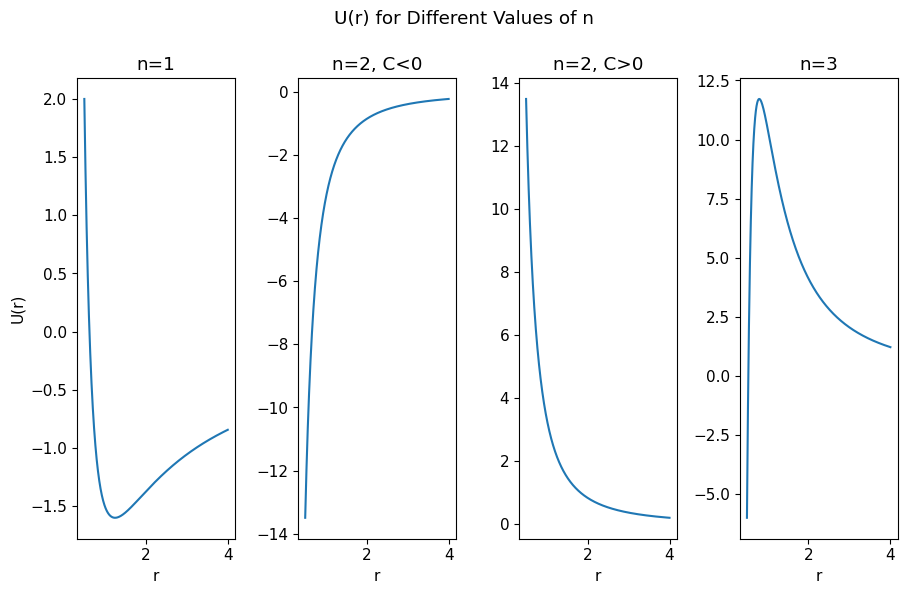
\includegraphics[width=0.8\textwidth]{U-plots}
    \caption{Plots of the shapes of potentials resulting from different values of n. The middle two are both the $n=2$ case, with the left one being with $C<0$ and the other with $C>0$. Note that for $n=1$, there is the characteristic potential well that symbolizes $r=p$. This is not present for $n=2$, but is for $n=3$ except concave down. }
    \label{fig:U-plots}
\end{figure}

Of course this doesn't just apply to integer values of  $n$. Looking at the plots, one might expect that $n<2$ produces stable equilibrium points, while $n>2$ would produce unstable equilibrium points. For this to be the case it needs to be that for $n<2$,  
\[
\frac{d^2U_n}{dr^2}\bigg|_{r=p_n}=\frac{3l^2}{\mu p_n^{4}}-\frac{n(n+1)\alpha_n}{p_n^{n+2}}>0\implies p_n^{2-n}<\frac{3l^2}{\mu\alpha_n n (n+1)}
.\]
Plugging in our equation for $p_n$ to this equation gives confirms that 
\[
p_n^{2-n}=\frac{l^2}{n\alpha_n\mu}< \frac{3}{n+1} \frac{l^2}{n\alpha_n\mu}  \text{ (for $n<2$)}
\]
as required for $p_n$ to be a stable equilibrium point. In the exact same vein (essentially just switching the directions of inequality), we can show that $n>2$ produces unstable equilibrium: 
\[
\frac{d^2U_n}{dr^2}\bigg|_{r=p_n}=\frac{3l^2}{\mu p_n^{4}}-\frac{n(n+1)\alpha_n}{p_n^{n+2}}<0\implies p_n^{2-n}>\frac{3l^2}{\mu\alpha_n n (n+1)}
.\]
Again plugging in the equilibrium point: 
\[
p_n^{2-n}=\frac{l^2}{n\alpha_n\mu}> \frac{3}{n+1} \frac{l^2}{n\alpha_n\mu}  \text{ (for $n>2$)}
\]

\section{Trajectory}

Ideally one would like to be able to analytically solve for the trajectory of all of these alternate potentials, similarly to how we did in the $n=1$ case. To go about doing so, note that rearranging $l=\mu r^2\dot\phi$ and combining it with the fact that $E_{\text{rel}}=\frac{\mu \dot r^2}{2} +U_{\text{eff}}(r)\equiv E$ gives 
\begin{equation}\label{eq:traj}
d\phi=\frac{l}{\mu r^2}dt=\frac{l}{\mu r^2}\frac{\sqrt{\mu}dr }{\sqrt{ 2(E-U_\text{eff}(r))}}\implies\phi=\int \frac{ldr}{r^2\sqrt{2\mu\left( E-U_{\text{eff}}(r) \right) } }
.\end{equation}
Unfortunately, this integral turns out to be impossible to analytically solve for almost all values of $n$. While it's difficult to show this rigorously, it was attempted with an integral calculator for a good amount of time and no solutions were present. The only exceptions to this were the $n=1$ and $n=2$ case. Then $n=1$ case is of course gravity's actual potential, which we've already solved. The $n=2$ case is different, but luckily still able to be tackled analytically. 

\subsection{Case $C>0$}

For now assume that $C>0$, although we will see shortly that $C<0$ is handled in somewhat similar manner. For $n=2$ the effective potential is $U_{\text{eff}}=\left( \frac{l^2}{2\mu}-\alpha_2 \right)\frac{1}{r^2}\equiv \frac{C}{r^2}$. Thus the integral we are trying to solve is 
\[
\phi=\int \frac{ldr}{r^2\sqrt{2\mu\left( E-C /r^2 \right) } }
.\]
Let $u=\frac{1}{r}$. Then $du=-\frac{1}{r^2} dr$: 
\[
\phi = -\frac{l}{\sqrt{2\mu} }\int \frac{du}{\sqrt{E-Cu^2} }
.\]
Since we're assuming for now that $C>0$, let $u^2=\frac{E}{C}\cos^2 x$. Then $u=\sqrt{\frac{E}{C}}\cos x\implies du=-\sqrt{\frac{E}{C}}\sin x$ (there's no problem taking the square root since $C>0$). Substituting, we get
\[
\phi=-\frac{l}{\sqrt{2\mu} }\int \frac{-\sqrt{\frac{E}{C}}\sin x }{\sqrt{E} \sqrt{1-\cos^2x} }=\frac{l}{\sqrt{2\mu C}}x
.\]
Combining this with the fact that $u=\sqrt{\frac{E}{C}}\cos x=\frac{1}{r}$, we get that
\[
\frac{1}{r}=\sqrt{\frac{E}{C}}\cos\left( \frac{\sqrt{2\mu C}}{l}\phi  \right)  
.\]
We can clean up slightly by expanding $C$ back out in terms of its components and defining $p_2=\sqrt{\left|\frac{C}{E}\right|} $. 
\begin{equation}\label{eq:C>0}
\frac{p_2}{r}=\cos\left( \sqrt{1- \frac{2\mu\alpha_2}{l^2}} \phi \right) 
.\end{equation}
Note that it's very tempting to look at the $\left( \frac{l^2}{\mu\alpha_2} \right)^{-1} $ in the cosine and try and notice that it happens to be $p_1^{-1}$, and then confuse yourself with the units (inside the square root should have no units, not $\text{m}^{-1}$). However $\alpha$ is defined differently in the $n=1$ and $n=2$ case, as $G_1$ and $G_2$ have different units, so the claim of significance for $ p_1$ showing up in the $n=2$ case isn't altogether clear. %Instead, define $e_2=\sqrt{1-\frac{2\mu\alpha_2}{l^2}}  $. Of course both $e_2$ and $p_2$ are defined quite differently here than in the $n=1$ case, but in some sense they both still match the units and functionality of their counterparts. For example $e_2=0$ still produces a circular orbit, as 


Unfortunately, although this is a nice closed form expression similar to that of $\frac{p}{r}=1+e\cos\phi$ as we found in the $n=1$ case, this can't easily be rendered any simpler since there is a coefficient inside the $\cos$ this time (in the $n=1$ case we used the fact that $x=r\cos\phi$ to cleanly change to Cartesian coordinates). However we can still plot such trajectories numerically, as can be seen in figure \ref{fig:trajectories}. It appears like a hyperbola, with a rapid turnaround near the origin and asymptotes as $r\to \infty$. Also here the physical interpretation of $p_2$ is clear: it represents the shortest distance between the trajectory and origin, i.e. the shortest distance possible between the two objects given an initial energy. 

\subsection{Case $C<0$}

We should also consider the case where $C<0$. If it is then we can instead define $u^2=-\frac{E}{C}\sinh^2x$. Then we have $u=-\sqrt{\frac{E}{-C}}\sinh x \implies du=-\sqrt{\frac{E}{-C}} \cosh x$ (we can take the negative value in the square root since this just represents the trajectory going the other way) and plugging in this substitution as we did before we arrive at 
\[
\phi = -\frac{l}{\sqrt{2\mu} }\int \frac{-\sqrt{\frac{E}{-C}} \cosh x}{\sqrt{E} \sqrt{1+\sinh^2 x}}dx=\frac{l}{\sqrt{-2\mu C}}x
.\]
Putting this back with the definition of $u$ gives 
\[
\frac{1}{r}=\sqrt{\frac{E}{-C}} \sinh\left( \frac{\sqrt{-2\mu C}}{l}\phi \right) 
.\]
Cleaning up to make this equation look like equation \ref{eq:C>0}: 
\begin{equation}\label{C<0}
\frac{p_2}{r}=\sinh\left( \sqrt{\frac{2\mu\alpha_2}{l^2}-1} \phi \right) 
.\end{equation}
This is even harder to physically interpret than equation \ref{eq:C>0}, but a numerically calculated trajectory can be seen in figure \ref{fig:trajectories}. The relative distance very quickly spirals inward, since the conservation of angular momentum is overcome by the gravitational potential that grows at the same rate. Also here the physical interpretation of $p_2$ isn't as clear cut as $C>0$.  

\begin{figure}[htpb]
    \centering
    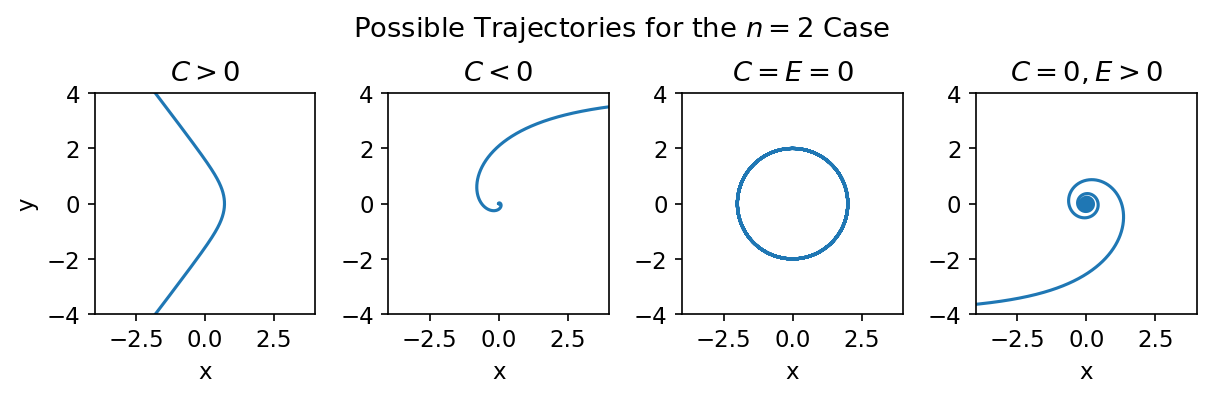
\includegraphics[width=0.8\textwidth]{trajectories}
    \caption{Plots of the trajectories for the $n=2$ case with $C>0$, $C<0$, $C=E=0$ and $C=0,E>0$. The initial conditions were all chosen arbitrarily and scaled to appear better when graphed, so the relative magnitude of each isn't comparable. }
    \label{fig:trajectories}
\end{figure}

\subsection{Case $C=0$}

For the $C=0$ case, equation \ref{eq:energy} reduces to $E=\frac{\mu \dot r^2}{2}+U_{\text{eff}}(r)=\frac{\mu\dot r^2}{2}$. Thus we have that $E\geq0$, but because equation \ref{eq:traj} requires $E\neq 0$ we have two cases to consider. 

\subsubsection{Case $E=0$}

Before looking at the more interesting cases, we must first consider the most boring possibility: $C=E=0$. By definition we have $E=\frac{\mu \dot r^2}{2}+U_{\text{eff}}(r)=\frac{\mu\dot r^2}{2}=0$, which implies $\dot r=0\implies r=r(0)$. Thus $C=E=0$ yield trajectories that are circles with whatever radius their initial conditions start them with. %To find the period of the orbit, recall Kepler's second law, which despite having been derived in the context of $n=1$ is potential--independent. Since the total area swept out is $\pi r^2$, we get that 
% \[
% \frac{\pi r^2}{T}=\frac{l}{2\mu}=
% .\]
% \[
% T=\frac{2\pi r(0)}{r\dot\phi}=\frac{2\pi \mu r(0)^2}{l}
% .\]

\subsubsection{Case $E> 0$}

If $C=0$ then equation \ref{eq:traj} becomes far simpler (throwing away integration constants as before): 
\[
\phi = \int \frac{ldr}{r^2\sqrt{2\mu E} }
\]
\begin{equation}\label{eq:c=0}
\implies\phi=-\frac{l}{\sqrt{2\mu E} } \frac{1}{r}
.\end{equation}
Intuitively what equation \ref{eq:c=0} represents (assuming initial conditions causing no constant terms) is that as the two objects' relative mass gets close to zero, $\phi$ gets very large which represents the trajectory spiraling quickly inward. As $r$ gets larger, phi approaches zero. This can seen graphically in figure \ref{fig:trajectories}, where the characteristic spiral inwards can be seen. It is interesting to note how much slower (in the physical distance sense, not the time sense) the $C=0$ spirals inward compared to the $C<0$ case. The reason for this is that the radial velocity is linear for $C=0$ as will be showed shortly, so $\phi$ changes more over the course of the fall inward/outward. 

One other interesting aspect of the $C=0$ case is that, unlike the $C\neq 0$ case, solving for the trajectory in terms of time is simple. Recall that for this system we already have an effective Lagrangian to solve: 
\[
\mathcal L_{\text{rel}}=T_{\text{rel}}-U_{\text{eff}}=\frac{\mu \dot r^2}{2}-\frac{C}{r^2}=\frac{\mu \dot r^2}{2}
.\]
Calculating the Euler--Lagrange equations: 
\[
\frac{d}{dt}\left( \frac{\partial \mathcal L}{dr} \right)= \mu \ddot r=\frac{\partial\mathcal L}{\partial r}=0\implies r=r(0)+\dot r(0)t
.\]
In a sense this is reasonable, since $C=0$ represents an effective potential of zero which causes the two bodies' relative distance to behave as a free particle. Of course for actual physical objects the motion would of course have to be stopped at some point physically by a collision. However ignoring this possibility and considering the two objects as point masses does lead to a moderately interesting result when you consider the relative perpendicular (i.e. non radial) velocity of the two bodies: 
\[
v_{\perp}(t)=r\dot\phi=r \frac{d}{dt}\left( -\frac{l}{r\sqrt{2\mu E} } \right)=\frac{1}{r\sqrt{2\mu E} }=\frac{1}{\sqrt{2\mu E} } \frac{1}{r(0)+\dot r(0)t}
.\]
Thus if the initial conditions are such that $\dot r(0)<0$, there will be a singularity and the particle will have infinite velocity in finite time. This also occurs in the $n=1$ case for radial velocity if you set two point masses at rest and set them on a collision course, but it's somewhat more interesting here because it's not the radial velocity that's going to infinity (indeed, it is constant) but instead the tangential velocity that is unbounded. 

\section{Discussion}

Overall, I believe the analysis presented here was successful and gives both a good qualitative sense of how these alternate potentials would behave as well as analytic predictions for their trajectories. Especially for the solutions to the $n=2$ case, going into this project it wasn't expected that they could be actually solved, so the fact that they can be was a pleasant surprise, even if they don't reduce quite as nicely as the $n=1$ case. 

One enjoyable part of the project is that throughout the analysis there were many interesting facts about how these other potentials that, while not violating any fundamental laws of physics, seem quite unintuitive to someone used to the $n=1$ case. For example the fact that when $C=0$ one can get infinite tangential velocity in finite time while maintaining finite radial velocity is extremely strange. It's simply something that doesn't happen when all orbits are ellipses/parabolas/hyperbolas which makes it quite satisfying when you notice something like it. 

Of course there is more that can be done on this topic. While it's unlikely that any of the other potentials can be solved analytically in general, there are surely some special cases for which interesting orbits could occur for other values of $n$. Also even if they're not analytic, solving them numerically could yield some interesting results. We already saw there there is somewhat of a dividing line between $n<2$ and  $n>2$ representing the transition between stable and unstable orbits, so analyzing some $n>2$ would show what orbits look like in the unstable regime. Likely they would be spirals inward and outward unless starting exactly at the equilibrium distance, but the calculations would have to be done to know for sure. 

\section{Conclusion}

The consequences of a hypothetical $U(r)=\frac{\alpha_n}{r^{n}}$ gravitational potential in the two body problem has been investigated. For the general $n\in\mathbb{R}$ case the equilibrium distances and their stability were found. To solve for trajectories analytically, the $n=2$ case was focused on and analytic solutions to all possible initial conditions were found. In addition these trajectories were numerically implemented to get a sense of their qualitative behavior. 




\end{document}
